\documentclass{beamer}
\usepackage{mathrsfs} %Pretty fonts
\usepackage{amsmath}
\usepackage{amssymb}
\usepackage{amsfonts}
\usepackage{amsthm}
\usepackage{bbm}
\usepackage{tikz}
\usetikzlibrary{arrows,shapes,positioning}
\usepackage{url} % insert Urls in bib


\bibliographystyle{plain}
\setbeamertemplate{bibliography item}{\insertbiblabel}


\newtheorem{proposition}{Proposition}[section]

\mode<presentation>{\usetheme{Madrid}}
%%%% COMMANDS %%%%
\usepackage{xifthen}

% Real Numbers
\newcommand{\RNums}{\mathbb{R}}
% sigma-algebra
\newcommand{\salg}{\sigma\text{-algebra}}
% borel sigma-algebra
\newcommand{\borelsalg}{\mathscr{B}(\RNums)}
% Indicator function
\newcommand{\ind}{\mathbbm{1}}
% F: Sigma Algebra
\newcommand{\salgF}{\mathscr{F}}
% Probability P (P measure)
\newcommand{\Pm}{\mathbb{P}}
% Expectation's E
\newcommand{\E}{\mathbb{E}}
%Expectation with Braces
\newcommand{\Exp}[1]{\E\left[#1\right]}
% Variance
\newcommand{\V}{\mathbb{V}}
%Variance  with Braces
\newcommand{\Var}[1]{\V\left[#1\right]}
% Continuous time stochastic process
\newcommand{\ctspr}{\{X_t\}_{t\geq 0}}
% Discrete time stochastic process
\newcommand{\dtspr}{\{X_n\}_{n\geq 0}}
% Insert only one number in the "align" environment
\newcommand\numberthis{\addtocounter{equation}{1}\tag{\theequation}}
% Measure Space
\newcommand{\MeasureSpace}[1]{(\Omega, \salgF, #1)}
% Proabability Space
\newcommand{\ProbSpace}{\MeasureSpace{\Pm}}
% Norm
\newcommand{\norm}[1]{\left\lVert#1\right\rVert}
% Inner Product
\newcommand{\innerprod}[2]{\langle #1, #2\rangle}
% Family N of processes between a and b
\newcommand{\Nfam}[2]{\mathcal{N}\left[#1, #2\right]}
% Family M of processes between a and b
\newcommand{\Mfam}[2]{\mathcal{M}\left[#1, #2\right]}
%Change of Brownian motion
\newcommand{\DeltaW}[1][]{%
\ifthenelse{\isempty{#1}}{\Delta W_i}{\Delta W_#1}%
}
% differential w.r.t. the brownian motion
\newcommand{\dW}[1][]{%
\ifthenelse{\isempty{#1}}{dW}{dW_#1}%
}
% n-th partial derivative w.r.t. a single variable
\newcommand{\partialwrt}[3][]{
\ifthenelse{\isempty{#1}}
{\frac{\partial #2}{\partial #3}}
{\frac{\partial^{#1} #2}{\partial #3^{#1}}}
}

% Big-oh notation
\newcommand{\bigO}{\mathcal{O}}

% Market
\newcommand{\market}{\{X(t)\}_{t\in[0,T]}}

\title{Theoretical Grounds for the valuation of European Options}
\author{Gerardo Dur\'an Mart\'in}
\institute{Universidad Marista}

\logo{
\includegraphics[height=1.7cm]{UMA_logo}}

\begin{document}
%Generates the title page
\frame{\titlepage}

\begin{frame}
	\frametitle{The Main Problem}
	How does one go about understanding the variations to derive Black-Scholes formula for vanilla options at a reachable level as to both comprehend theory and intuition?
	\begin{equation}
		\partialwrt{C}{t} + \frac{1}{2}\sigma^2S^2\partialwrt[2]{C}{S} + rS\partialwrt{C}{S} - rC = 0.
	\end{equation}
\end{frame}

\begin{frame}
	\frametitle{Raison d'\^etre}
	\begin{enumerate}
		\item<1-> \textit{Plain vanilla} option pricing play an important part in the derivatives' market;
		\item<2-> option pricing is mainly presented as a deeply esoteric subject that is either too deep to delve into, or a complex one that requires a profound understanding in stochastic-calculus and analysis;
		\item<3-> to present the theory in a robust yet, accessible level for an undergraduate; and
		\item<4-> inquisitiveness.
	\end{enumerate}
\end{frame}

%% Instruments
\begin{frame}
\frametitle{The Objectives}
	\begin{columns}[c]	
	
	\column{0.45\textwidth}
	\begin{itemize}
		\item <1-| alert@1> Review of Financial Markets and the Instruments therein.
		\item <2-| alert@2> Review of probability Theory and Stochastic Processes
		\item <3-| alert@3> Option Pricing in Discrete Time
		\item <4-| alert@4> Introduction to the Brownian Motion
		\item <5-| alert@5> Introduction to Stochastic Calculus
		\item <6-| alert@6> Option Pricing in Continuous Time
	\end{itemize}
	
	\column{0.5\textwidth}
	\only<1>{
	what markets are; the participants; and instruments in this market. We present derivatives, the main driver of this work.
	\begin{figure}[h]
	\centering
	\label{fig:call_option_payoff}
	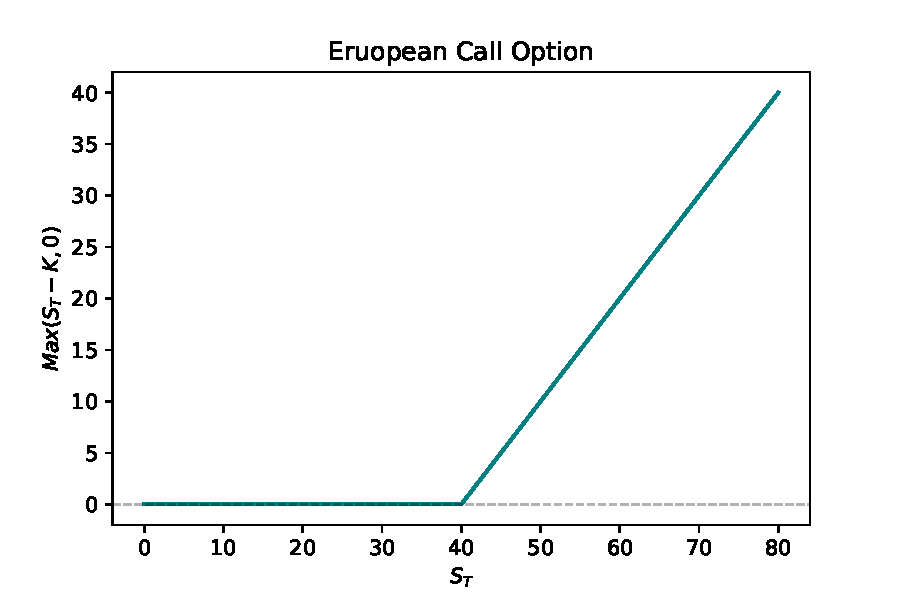
\includegraphics[width=0.7\textwidth]{../images/Call.pdf}	
	\caption{European Call Payoff}
	\end{figure}

	}
	\only<2>{
	\begin{figure}[h]
		\centering
		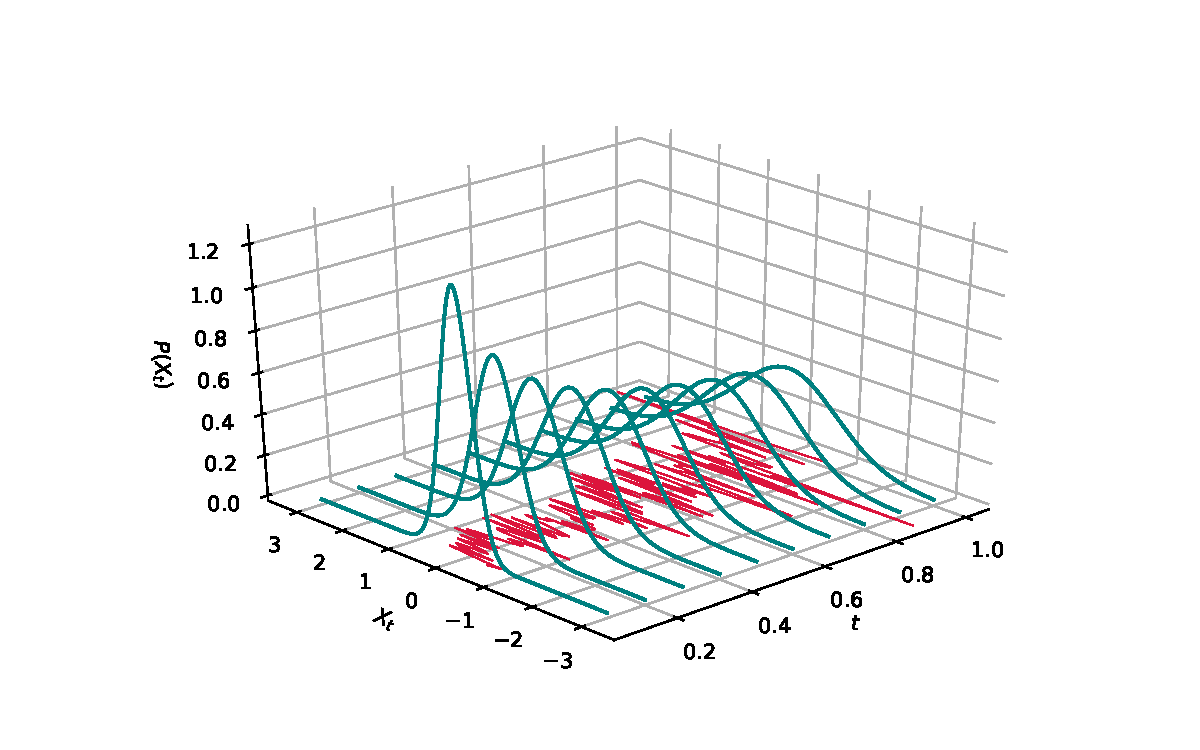
\includegraphics[width=0.90\textwidth]{../images/stoch_process_3d}
		\caption{Distribution and Path of a Stochastic Process.}
		\label{fig:stochastic_process}
	\end{figure}
	}
	
	\only<3>{
	\begin{figure}[h]
	\centering
	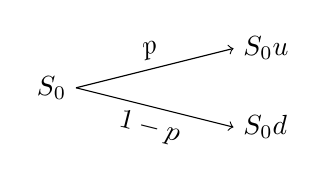
\begin{tikzpicture}
	    \draw[->] (0,0) node[left]{$S_0$} --(2, 0.5) node[pos=0.5, sloped, above] {$p$};
	    \node[right] at (2, 0.5) {$S_0u$};
	
	    \draw[->] (0,0) --(2, -0.5) node[pos=0.5, sloped, below] {$1-p$};
	    \node[right] at (2, -0.5) {$S_0d$};
	\end{tikzpicture}
	\caption{Possible path of the stock after one unit of time.}
	\end{figure}
	}

	\only<4>{
	\begin{figure}[h]
		\centering
		\includegraphics[width=0.9\textwidth]{../images/bm}
		\caption{Sample Paths of a Brownian Motion}
		\label{fig:Brownian_Motion}
	\end{figure}
	}
	\only<5>{
	\begin{figure}[hbt]
	  \includegraphics[width=0.9\textwidth]{../images/simple_process}
	  \caption{Simulation of Simple Process}
	\end{figure}
	}
	
	\only<6>{
	\begin{figure}[h!]
	  \includegraphics[width=0.90\textwidth]{../images/european_call_montecarlo}
	  \label{fig:montecarlo_simulation}
	  \caption{250 simulation of a European Call under $\Qm$.}
	\end{figure}
	}
	\end{columns}
\end{frame}

\begin{frame}
	\frametitle{Chapters}
	\begin{enumerate}
		\item Financial Markets
		\item Probability Theory
		\item A Primer on Pricing
		\item $L_2$ Spaces and the Brownian Motion
		\item Stochastic Calculus
		\item Option Pricing
	\end{enumerate}
\end{frame}


\begin{frame}
	\frametitle{The Results}
	We derived the Black-Scholes PDE via replication argument:
	\begin{equation}
	\partialwrt{C}{t} + \frac{1}{2}\sigma^2S^2\partialwrt[2]{C}{S} + rS\partialwrt{C}{S} - rC = 0.
	\end{equation}
	It was shown that, in general, for an attainable claim, the price of the claim at $t=0$ is.
	\begin{equation}\label{eq:risk-neutral-expectation}
	  c = \ExpMeasure{\Qm}{\nu(T)g(S_T)}
	\end{equation}
\end{frame}

\begin{frame}
	\frametitle{Results}
	\framesubtitle{Cont'd}
	For the case of a call option, we derived the closed formula for its price
	\begin{equation} \label{eq:risk-neutral-price}
		c = S_0 \Phi(d_+) - Ke^{-rT}\Phi(d_-)
	\end{equation}
\end{frame}

\begin{frame}
	\frametitle{Results}
	\framesubtitle{Cont'd}
	Using the Feynman-Kac formula, it was shown that
	\begin{equation}
		\partialwrt{C}{t} + \frac{1}{2}\sigma^2S^2\partialwrt[2]{C}{S} + rS\partialwrt{C}{S} - rC = 0 \Rightarrow \ExpMeasure{\Qm}{\nu(T)g(S_T)}.
	\end{equation}
\end{frame}


\begin{frame}
	\frametitle{Results}
	\framesubtitle{Cont'd}
	We converged to the price of a call option using Montecarlo methods.
		\begin{figure}[h]
		\centering
	  \includegraphics[width=0.5\textwidth]{../images/montecarlo_distribution}
	  \caption{Mean distribution of a simulated call option.}
	\end{figure}
\end{frame}


\begin{frame}[allowframebreaks]
\tiny
\nocite{*}
\bibliography{../misc/ref}
\end{frame}
\end{document}